\chapter{Gr\'aficos.}




\section{Las ecuaciones de Lotka y Volterra.}

En esta secci\'on vamos a estudiar un modelo cl\'asico para una situaci\'on depredador presa.
Este modelo  fue ideado alrededor del a\~no 1920 por el matem\'atico italiano Vito Volterra,
(1860-1940) y, desarrollado independientemente en la misma \'epoca,  por el biof\'{\i}sico
austr\'{\i}aco Alfred James Lotka, (1880-1940).

Volterra estudiaba las variaciones peri\'odicas observadas en las poblaciones de tiburones y
sus peces-alimento en el Mar Adri\'atico.

Sea $x(t)$ el n\'umero de presas y sea  $y(t)$ el n\'umero de depredadores en el instante $t$.
En este modelo se supone lo siguiente:


\begin{equation}\label{especies3}
\left\{ \begin{aligned}
\dot{x} & = A \, x - B\, x \, y, \\
\dot{y} & = - C\,  y  + D \, x \, y ,
\end{aligned} \right.
\end{equation}
donde $A$, $B$, $C$ y $D$ son constantes positivas.

 Este sistema de ecuaciones, que a simple vista se parece a los que hemos estudiado, no
es nada sencillo. No es posible hallar sus soluci\'on de manera expl\'{\i}cita, mediante
m\'etodos num\'ericos es posible aproximar sus soluciones.

Consideremos el siguiente caso particular

\begin{equation}\label{especies4}
\left\{ \begin{aligned}
\dot{x} & =  x - x \, y, \\
\dot{y} & = (0,3)\, x \, y  -  (0,3)  \, y ,
\end{aligned} \right.
\end{equation}
con condici\'on inicial $$x(0) = 2 \qquad \qquad y(0) = 2.$$

Suponemos que $x$ e $y$ representan al n\'umero de presas y depredadores, contadas en miles de
individuos y $t$ es el tiempo medido en semanas.

En la siguiente figura tenemos los gr\'aficos de las soluciones.



\begin{figure}
\scalebox{.80}{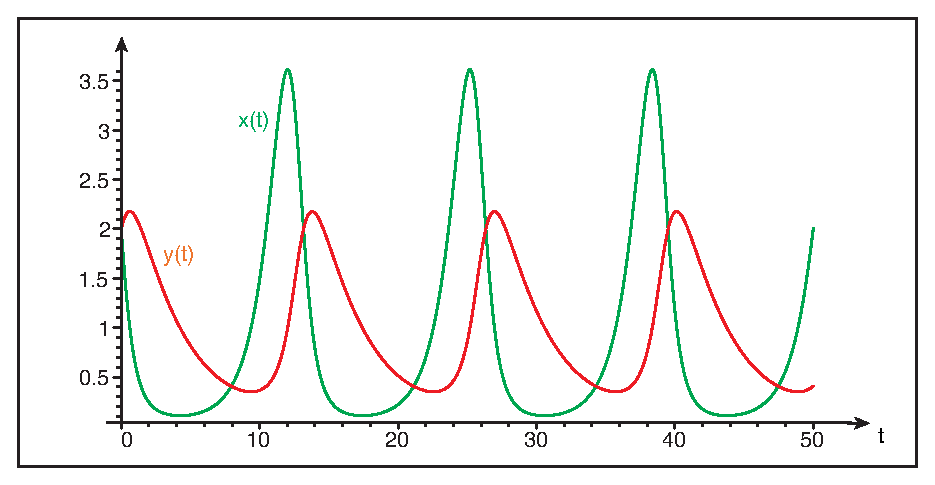
\includegraphics{especies4(LV).eps}}  \caption{Comportamiento del sistema para
$0 \leq t \leq  50 $}\label{f1}
\end{figure}

Se observa que el n\'umero de presas y de depredadores comienza a disminuir muy r\'apidamente
hasta casi extinguirse, con cierto desfase entre presas y depredadores. En el momento en que
hay muy pocos depredadores comienza a aumentar el n\'umero de presas y despu\'es el n\'umero
de depredadores alcanz\'andose valores m\'aximos con desfase y entrando en un ciclo que se
repite.

La siguiente figura muestra la trayectoria correspondiente.

\begin{figure}
\scalebox{.90}{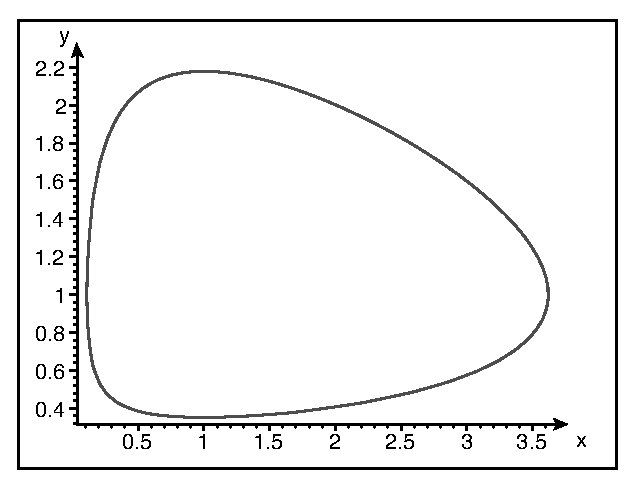
\includegraphics{especies5(LV).eps}}  \caption{Trayectoria del
sistema}\label{f2}
\end{figure}

\pagebreak

\section{Superficies.}

Sea $f(x, y) = x^2 - y^2$ entonces las curvas de nivel de $f$ son los conjuntos en los que
$x^2 - y^2 = c.$ Estos conjuntos nos dan una idea de como es el gr\'afico de $f$.


\begin{figure}
\begin{tabular}{c c}
\scalebox{.80}{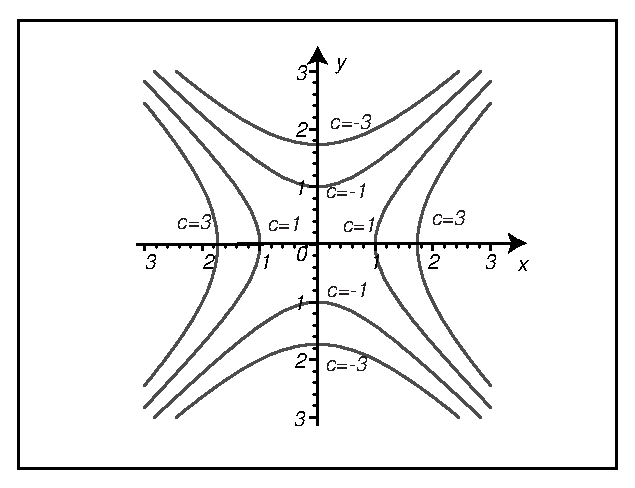
\includegraphics{nivelsilla1.eps}}  &
\scalebox{.80}{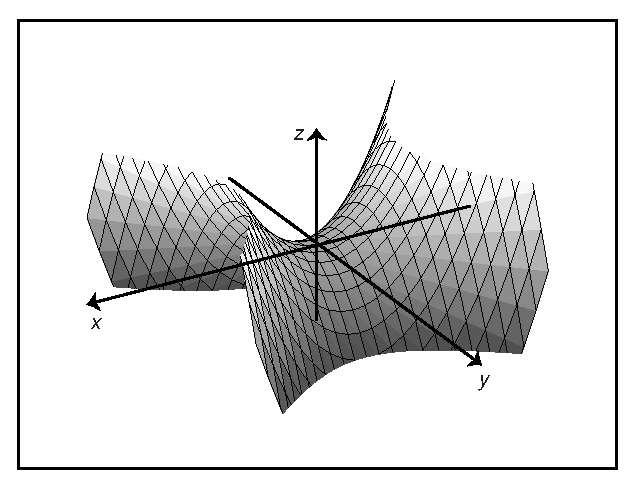
\includegraphics{silla1.eps}}
\end{tabular} \caption{curvas de nivel y gr\'afico de $f(x, y) = x^2 - y^2$}\label{f3}
\end{figure}
Esta superficie se conoce con el nombre de paraboloide hiperb\'olico  o ``silla de montar''.
\index{paraboloide!hiperb\'olico}

\section{Elaboraci\'on de los gr\'aficos.}

En los ejemplos de este cap\'{\i}tulo hemos visto que para incorporar un gr\'afico al
documento es conveniente tener un archivo del tipo ``eps'' (encapsulated postscript).

Los archivos gr\'aficos que aparecen en este cap\'{\i}tulo fueron generados con Maple y
despu\'es editados con Illustrator de Adobe.

A continuaci�n describimos los comandos usados en Maple para generar los gr\'aficos.

\

Para generar la Figura \ref{f1} usar el siguiente comando:

\begin{verbatim}
>plotsetup(ps,plotoptions=`colour=cmyk,width=6in,height=3in`);
 fcns:={x(t),y(t)};
 odes:=diff(x(t),t)=x(t)*(1-y(t)),diff(y(t),t)=.3*y(t)*(x(t)-1);
 soln:=dsolve({odes[1],odes[2],x(0)=2,y(0)=2},{x(t),y(t)},type=numeric);
 with(plots):
 odeplot(soln,[[t,y(t)], [t,x(t)]],0..50, style=line, numpoints=1000);

\end{verbatim}

\

Para generar la Figura \ref{f2} usar el siguiente comando:

\begin{verbatim}
>with(plots):
implicitplot((0.3)*ln(x) - (0.3)*x + ln(y) - y = - 1.7 , x=0.1..4,
y=0.1..4,numpoints=5000);
\end{verbatim}

Para generar los dos elementos Figura \ref{f3} usar el siguiente comando:

\begin{verbatim}
>plot3d( x^2-y^2, x=-3..3, y=-3..3, axes=normal, labels=[x,y,z],
shading = ZGREYSCALE, style = PATCH, tickmarks=[0,0,0],
view=-3..3,orientation=[60,45]  );

with(plots):
> implicitplot({x^2 - y^2 = 1,x^2 - y^2 = 3, x^2 - y^2 = -1,x^2 - y^2 = -3},
x=-3..3,y=-3..3,scaling=constrained);


\end{verbatim}
